%==============================
\section{Uncertainty-aware Reactive Coordination under Dynamic Temporal Logic Tasks}
\label{ch06:sec:ch06_uncertain}

Recent {advances in computation, perception and communication
enable the deployment of autonomous robots in large, remote and hazardous environments,
such as offshore drilling platforms~\cite{shukla2016application}
and construction sites~\cite{bock2007construction}.
Concurrent motion and actions can greatly improve the team efficiency~\cite{toth2002overview, cliff2015online},
while direct collaboration on a single task further extends system capabilities~\cite{varava2017herding}.}
% fink2008multi,
% Temporal tasks as LTL formulas
To specify complex tasks beyond simple sequential visiting,
many studies employ formal languages such as Linear Temporal Logic (LTL)
formulas~\cite{baier2008principles}, as an intuitive yet powerful way to describe
both spatial and temporal requirements on the team behavior~\cite{kantaros2020stylus, guo2018multirobot}.
% schillinger2018simultaneous
However, while tasks are commonly defined over static features such as regions and landmarks,
many real-world applications involve dynamic targets, e.g., monitoring animal flocks
or tracking moving vehicles~\cite{robin2016multi}.
These scenarios pose particular challenges for traditional
offline methods that are designed for tasks over static features~\cite{luo2022temporal, sahin2019multirobot, Liu2024fproduct},
as the future motion of targets can significantly impact the performance
and even correctness of the overall plan.

This work proposes \textbf{UMBRELLA},
an online planning framework
for multi-robot coordination under dynamic temporal tasks.
It integrates CP-based motion prediction
with MCTS for task assignment.
Predicted target motions and quantified uncertainty
are used after ``Expansion'' to filter child nodes,
and incorporated into ``Simulation''
to evaluate partial plans
under the Conditional Value at Risk (CVaR) metric.
To handle online updates of target motions and newly released tasks,
a receding-horizon scheme is adopted to dynamically adjust task assignments.
The framework ensures satisfaction of LTL-specified spatial-temporal constraints
while accounting for target motion uncertainty,
The framework ensures LTL-specified spatial-temporal constraints while accounting for target motion uncertainty,
requiring only partial synchronization during collaborative task execution.
The framework ensures that the resulting execution satisfies the temporal and spatial constraints
specified by LTL formulas, while accounting for target motion uncertainty.
Only partial synchronization is required for collaborative tasks during online execution.
Compared with offline baselines assuming static workspaces or simple periodic replanning,
our method significantly reduces both the mean and variance of the average makespan.


The main contribution is two-fold:
(I) the incorporation of CP-based prediction into online multi-robot coordination under complex
temporal tasks associated with dynamic targets;
(II) a substantial reduction in the average makespan for temporal tasks
specified offline and released online,
with a $23\%$ and $71\%$ decrease in mean and variance, respectively.


\subsection{Problem Description}\label{ch06:sec:problem}

%==============================
\subsubsection{Robots and Targets}\label{ch06:subsec:robots}
Consider a team of~$N$ autonomous robots operating within a
workspace~$\mathcal{W}\subset \mathbb{R}^{3}$.
The state of robot~$n \in \mathcal{N} \triangleq \{1, \cdots, N\}$  at time \( t \)
is \(x_t \in \mathcal{W}\).
The maximum velocity of robot \(n\) is denoted by~$v_n$.
% Similar to the action model from~\cite{guo2016task},
Each robot $n$ can execute actions from a set~$\mathcal{A}_n$.
Let~$\mathcal{A}\triangleq\bigcup_{n\in\mathcal{N}}\mathcal{A}_n$.
The team is pre-programmed with collaborations~$\mathcal{C}\triangleq \{C_1,\cdots, C_k\}$,
where each collaboration $C_k\in \mathcal{C}$ consists of a list of actions
that must be executed by different robots, denoted by:
$C_k \triangleq \left[a_1,\,a_2,\cdots,a_{\ell_k}\right]$,
where~$\ell_k>0$ is the number of required actions,
and~$a_{\ell}\in \mathcal{A}$ for $\forall \ell=1,\cdots,\ell_k$.
Each action $a_{\ell}\in C_k$ should be performed by a capable robot~$n$,
i.e., $a_\ell\in \mathcal{A}_{n}$.
Each collaboration has a fixed duration~$\rho :\mathcal{C}\rightarrow \mathbb{R}_{+}$.

Moreover, the workspace contains \(M\) dynamic targets with unknown trajectories.
The position of target~\( m \in \mathcal{M} \triangleq \{1, \cdots, M\}\) at time~\( t \) is modeled
as a random variable~\( Y_{t,m} \in \mathbb{R}^{2} \),
with the joint target state~\( Y_t \triangleq \left(Y_{t,1}, \cdots, Y_{t,M}\right) \in \mathbb{R}^{2M} \).
Their trajectories are assumed to follow an unknown distribution~\( \mathcal{D} \),
i.e., \( \left(Y_{0}, Y_{1}, \cdots \right) \sim \mathcal{D} \).
A total of \( \bar{K} \) independent trajectory samples~\( Y^{(i)} \triangleq (Y_0^{(i)}, Y_1^{(i)}, \cdots) \)
are available,
partitioned into a calibration set~\( D_{\texttt{cal}} \triangleq \{ Y^{(1)}, \cdots, Y^{(K)} \} \)
and a training set~\( D_{\texttt{tra}} \triangleq \{ Y^{(K+1)}, \cdots , Y^{(\bar{K})} \} \).
The distribution~$\mathcal{D}$ is independent of robot behaviors,
i.e., it does not depend on the team state~$x$.
No assumptions are made about the form of the distribution $\mathcal{D}$,
but it is assumed that $\mathcal{D}$ is independent of the robot team,
as well as the availability of the training dataset~$\mathcal{D}_{\texttt{tra}}$
and the calibration dataset~$\mathcal{D}_{\texttt{cal}}$,
which are independently drawn from $\mathcal{D}$~\cite{Lars2023CP,Matthew2024CP},
for all potential dynamic targets.
Let $\mathcal{D}$ be an unknown distribution over target trajectories,
and let $\left(Y_{0}, Y_{1}, \cdots \right) \sim \mathcal{D}$
describe a random trajectory where the stacked target positions~$Y_{t}
\triangleq \left(Y_{t, 1}, \cdots, Y_{t, m}\right)$ at time $t$ is drawn from $\mathbb{R}^{2m}$.
Perfect observations of target positions and velocities are continuously available,
denoted by~$Y_{0:t} \triangleq \left(Y_{0}, \cdots, Y_{t}\right)$
and~$V_{0:t} \triangleq \left(V_{0}, \cdots, V_{t}\right)$,
where~$V_{t} \triangleq \left(V_{t,1}, \cdots, V_{t,M}\right)$.
% Let \(v^{\ast}_{m}(t)= \max \left\{ |V_{\varsigma , m}| : \varsigma \leq t \right\}\)
% denote the maximum velocity recorded for target \(m\) up to time \(t\).
A centralized scheme aggregates all measurements
and fuses them into real-time estimates of target states.
For simplicity, static task regions and obstacles are modeled as targets with zero velocity.


%==============================
\subsubsection{Task Specification}\label{ch06:subsec:task-specification}
Consider two types of atomic propositions:
(I) $p^m_n$ is \textit{true} if the distance between
robot $n \in \mathcal{N}$ and target $m \in \mathcal{M}$ is
below a given threshold.
Let $\textbf{p}\triangleq \{p^m_n,\, \forall m \in \mathcal{M},
n \in \mathcal{N}\}$;
% (II) $a^{k,m}_n$ is \textit{true} when robot~$n \in \mathcal{N}$
% performs a {local} action~$a_k\in \mathcal{A}_n^{\texttt{l}}$
% on target $m$.
% Let~$\textbf{a} \triangleq\{a^{k,m}_n,\forall m \in \mathcal{M},
% \forall a_k\in \mathcal{A}_n^\texttt{l}, n \in \mathcal{N}\}$;
(II) $c_k^{m}$ is \textit{true} if collaboration~$C_k$
is executed on target~\(m\).
Let $\textbf{c} \triangleq\{c_k^{m}, \forall m \in \mathcal{M},
\forall C_k \in \mathcal{C}, \forall a^c \in C_k\}$.
% For brevity, when the robot~$n$ in~$\textbf{p}$
% is set to ``all'', it indicates all robots should provide
% this action, and when set to ``any'', it means any robot can perform it.
Thus, the complete set of propositions is denoted by~$AP \triangleq \textbf{p} \cup \textbf{c}$.

Given these propositions,
a team-wise \emph{task} is represented as a {syntactically co-safe} LTL (sc-LTL) formula:
$\varphi_{i} = \text{sc-LTL}(AP)$.
The overall task specification is represented as a set of LTL formulas,
which consists of two parts:
\begin{equation}\label{ch06:eq:reactive-task}
  \varphi \triangleq \varphi_\texttt{static}
  \bigwedge_{\bar{e}\in \bar{E}} \Box \left( \varphi_\texttt{obs}^{\bar{e}}
  \rightarrow \Diamond\varphi_\texttt{rep}^{\bar{e}} \right),
\end{equation}
where~\(\varphi_\texttt{static}\) is a predefined set of sc-LTL formulas;
% as {syntactically co-safe} LTL (sc-LTL) over the propositions~$AP$;
$\bar{E}$ is the set of events triggered by online observations;
$\varphi_\texttt{obs}^{\bar{e}}$ is the propositional condition for event~$\bar{e}\in \bar{E}$;
and~$\varphi_\texttt{rep}^{\bar{e}}$ is the corresponding response task, also specified as sc-LTL.
Specifically, if $\varphi_\texttt{obs}^{\bar{e}}$ holds,
then $\varphi_\texttt{rep}^{\bar{e}}$ must eventually be satisfied.
We adopt the standard LTL syntax~\cite{baier2008principles}:
$\varphi \triangleq \top \;|\; p  \;|\; \varphi_1 \wedge \varphi_2  \;|
\; \neg \varphi  \;|\; \bigcirc \varphi  \;|\;  \varphi_1 \,\textsf{U}\, \varphi_2,$
where $\top\triangleq \texttt{True}$, $p \in AP$, $\bigcirc$ (\textit{next}),
$\textsf{U}$ (\textit{until}) and $\bot\triangleq \neg \top$.
% The full semantics and syntax of LTL are omitted here for brevity; see e.g., \cite{baier2008principles}.
sc-LTL~\cite{belta2017formal} is a fragment of LTL restricted to operators~\( \bigcirc \), $\textsf{U}$,
and $\Diamond$ (eventually), written in positive normal form without the
negation operator $\neg$ preceding temporal operators.


Moreover, the task plan for the robot team is defined as
\begin{equation}\label{ch06:plan}
    \Pi_{\mathcal{N}} \triangleq (\pi_1, \pi_2, \cdots, \pi_N),
\end{equation}
where \(\pi_n \triangleq (t^1_n,a^1_n,m^1_n)(t^2_n, a^2_n,m^2_n)
\cdots (t^{K_n}_n, a^{K_n}_n,m^{K_n}_n) \)
is the timed sequence of actions and corresponding targets for robot \(n\in \mathcal{N}\).
Each action \(a^k_n \in \mathcal{A}_n\) is executed on target \(m^k_n\in \mathcal{M}\)
at time~$t^k_n>0$,
where $k \in \mathcal{K}_n\triangleq \{1,\cdots, K_n\}$.
% with~$K_n>0$ being the length.
Given~$\Pi_{\mathcal{N}}$, the induced trace is given by the sequence of propositions
satisfied by the actions, i.e.,
\(w_\Pi = \sigma_1 \sigma_2 \cdots \sigma_L\)
where~\( \sigma_\ell \in 2^{\textit{AP}} \).
The language of~\( \varphi \) is
$\mathcal{L}_\varphi \triangleq \{\boldsymbol{w}\,|\,w\models\varphi\}$,
% $\mathcal{L}_\varphi \triangleq Words(\varphi) \triangleq
% \{\boldsymbol{w}\,|\,w\models\varphi\}$,
where $\models$ is the satisfaction relation.
Since sc-LTL formulas admit satisfaction by finite traces~\cite{belta2017formal,baier2008principles},
the plan satisfies \(\varphi\) if $w_\Pi\in \mathcal{L}_\varphi$, denoted by \(\Pi_\mathcal{N} \models \varphi\).
% it can be checked whether the trace derived from the plan \(\Pi_\mathcal{N}\)
% belongs to the language of~\(\varphi\), i.e., $w_\Pi\in \mathcal{L}_\varphi$.
% In this case, the task plan is said to satisfy~\(\varphi\)
% and denoted by~\(\Pi_\mathcal{N} \models \varphi\).
The \emph{makespan}~$T_\varphi$ is defined as the minimal time to generate a trace satisfying~$\varphi$.
As the tasks assigned to the robot system consist of initially issued tasks
and online triggered tasks during execution,
for a sequence of tasks $\varphi(t) \triangleq \{ \varphi_1, \ldots, \varphi_L \}$ received up to time~$t$,
the \emph{average makespan} is defined as:
$\overline{T}_\varphi \triangleq \frac{1}{L} \sum_{\ell = 1}^{L} T_{\varphi_\ell}.$

% The \textit{makespan} for robots to fulfill a task \(\varphi\), i.e.
% the time interval between when task \(\varphi\) is received and when it
% is satisfied is denoted by \(T_\varphi\).
% The tasks assigned to the robots consist of initially issued static tasks
% and online tasks triggered during execution.
% Thus, the average makespan of all tasks in~\eqref{ch06:eq:reactive-task} is denoted by:
% $\overline{T}_{{\varphi}} \triangleq \frac{\sum_{\ell=1}^{L_t} T_{\varphi_\ell}} {L_t}$,
% where ${\varphi}(t)=\{\varphi_1,\cdots,\varphi_{L_t}\}$
% is the set of tasks known by time~$t\geq 0$.

%% %==============================
\subsubsection{Problem Statement}\label{ch06:subsec:prob-statement}

Given task formulas~$\varphi(t)$ and observations~$\{Y_{0:t}, V_{0:t}\}$,
the overall objective is to synthesize the team-wise plan~\(\Pi_\mathcal{N}\)
to satisfy~\(\varphi(t)\) and minimize
the average makespan~\(\overline{T}_{\varphi}\).
%% \begin{problem}\label{ch06:prob:formulation}
%% Given the task specification in~\eqref{ch06:eq:reactive-task} and
%% real-time observations of the environment,
%% synthesize the plan \(\Pi_\mathcal{N}\) for the robot team
%% to satisfy \(\phi(t)\) and minimize the average makespan~\(\overline{T}_{\phi}\).
%%
%% \end{problem}
%====================
\begin{example}\label{ch06:exp:task}
Consider a fleet of UAVs and ground robots (GRs) deployed for wildlife monitoring
in a workspace labeled with \texttt{poacher}, \texttt{trap} and \texttt{animal}.
An offline collaborative task~$\varphi_\texttt{1}$ is specified as:
\begin{equation}
\label{ch06:eq:task}
\begin{aligned}
    \varphi_\texttt{1} = \varphi_{\texttt{p}-\texttt{s}_1} \wedge \varphi_{\texttt{mf}-\texttt{a}}, \:
    \varphi_{\texttt{p}-\texttt{s}_1} = \Diamond \texttt{patrol}_{\texttt{s}_1},\\
    \varphi_{\texttt{mf}-\texttt{a}} = \Diamond(\texttt{monitor}_\texttt{a}\wedge\neg\texttt{film}_\texttt{a}\wedge\Diamond\texttt{film}_\texttt{a}), \\
    % \varphi_\texttt{1} \! = \! \Diamond \texttt{patrol}_{\texttt{s}_1} \! \wedge
    % \Diamond(\texttt{monitor}_\texttt{a}\wedge\neg\texttt{film}_\texttt{a}\wedge\Diamond\texttt{film}_\texttt{a}),
\end{aligned}
\end{equation}
which requires to patrol region \(\texttt{s}_1\),
monitor and film antelopes in sequence.
GRs must avoid obstacles in the workspace.
The reactive protocol specifies:
$(\texttt{poacher}\rightarrow\Diamond \texttt{arrest})$,
where an ``arrest'' task is triggered upon detecting a poacher,
and $(\texttt{trap}\wedge\texttt{animal}\rightarrow\Diamond \texttt{rescue})$,
triggers a ``rescue'' task when an animal is trapped.

\end{example}
%======================================

%==============================
\begin{figure*}[!t]
  \centering
  %\color{blue}
  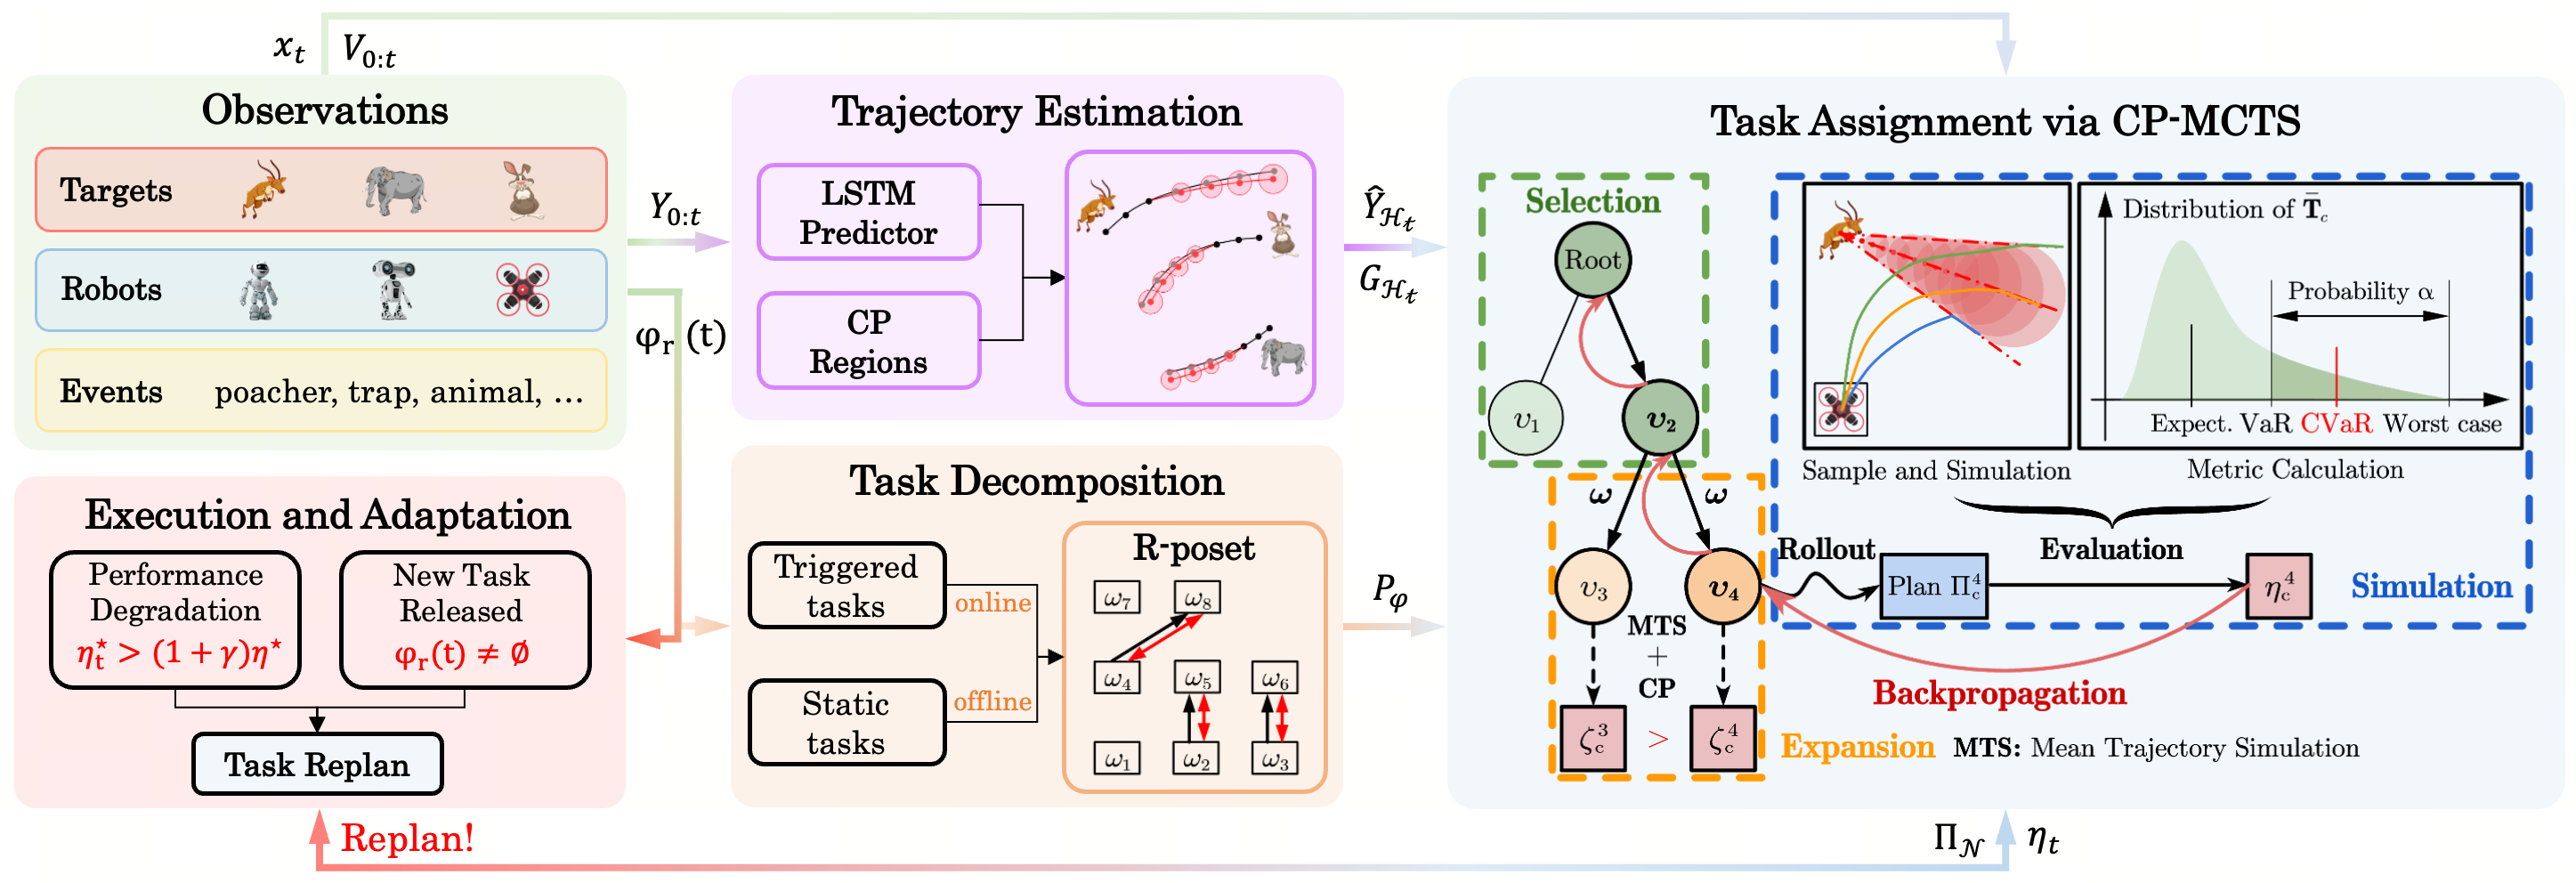
\includegraphics[width=7.0in]{figures/ch06/new-framework.png}
  \vspace{-6mm}
  \caption{Overview of the proposed framework,
  consisting of four main components:
  (i) trajectory estimation via LSTM and CP,
  (ii) task decomposition into an R-poset,
  (iii) CP-MCTS for uncertainty-aware assignment,
  and (iv) online execution and receding-horizon adaptation.
  In the R-poset illustration,
  precedence and mutual-exclusion relations are marked by black and red arrows,
  respectively.}
  \label{ch06:fig:fra}
  \vspace{-0.2in}
\end{figure*}
%==============================



%==============================
\subsection{Trajectory Estimation of Dynamic Targets}\label{ch06:subsec: trajectory}

\subsubsection{Trajectory Predictor}
Given a task horizon~$T_{{\varphi}}$ and the history of target observations $Y_{0:t}$,
we train an independent trajectory predictor for each target
based on the training dataset~$D_{\texttt{tra}}$.
% For target $m \in \mathcal{M}$,
Let $D_{\texttt{tra}}^m \subset D_{\texttt{tra}}$ collect trajectories of target~$m$,
$Y_{0:T,m}^{(i)} \triangleq (Y_{0,m}^{(i)}, \cdots, Y_{t,m}^{(i)}, Y_{t+1,m}^{(i)}, \cdots, Y_{T_{{\varphi}},m}^{(i)})$
denotes the $i$-th trajectory in $D_{\texttt{tra}}^m$.
The trajectory predictor is defined as
$\Upsilon_m : \mathbb{R}^{2(t+1)} \rightarrow \mathbb{R}^{2(T_{{\varphi}}-t)}$ that estimates the future states of target $m$
% $ \left(Y_{t+1,m},\cdots, Y_{T_{{\varphi}},m}\right)$
as $\widehat{Y}_{\mathcal{H}_t,m} \triangleq \Upsilon_m (Y_{0:t,m}),
\mathcal{H}_t \triangleq \{t+1, \cdots, T_{{\varphi}}\}$, where
$\Upsilon_m (Y_{0:t,m}) \triangleq (\widehat{Y}_{t+1 \mid t,m}, \cdots, \widehat{Y}_{T_{{\varphi}} \mid t,m})$.
Let $\mathbf{\Upsilon} \triangleq (\Upsilon_1, \cdots, \Upsilon_M)$.
In principle, any trajectory predictor can be employed,
including long short-term memory (LSTM) networks~\cite{Hochreiter1997LSTM}, recurrent neural networks (RNN)~\cite{rnn}, and gated recurrent units (GRU)~\cite{gru}.
% transformer architectures \cite{Nayakanti2023Transformer}.
% To train $\Upsilon_m$ for each target $m$, the training dataset~$D_{\texttt{tra}}^m$
% contains trajectory data for target $m$, i.e.,
% $Y_{0:T,m}^{(i)} \triangleq (Y_{0,m}^{(i)}, \cdots, Y_{t,m}^{(i)}, Y_{t+1,m}^{(i)}, \cdots, Y_{T_{{\varphi}},m}^{(i)})$
% is the $i$-th trajectory of target $m$ in the dataset~$D_{\texttt{tra}}^m$.
In this work, a LSTM network is adopted for each target and trained
by minimizing the following loss function:
$$\underset{\Upsilon_m}{\textbf{min}} \frac{1}{|D_{\texttt{tra}}^m|} \sum_{i=1}^{|D_{\texttt{tra}}^m|} \left\| Y_{\mathcal{H}_t,m}^{(i)} - \Upsilon_m(Y_{0:t,m}^{(i)}) \right\|^2,$$
which is the Mean Squared Error (MSE) over the predicted trajectory for target $m$.
% The overall prediction for all targets is then obtained by combining the individual predictions:
Stacking per-target predictions gives
$\widehat{Y}_{\mathcal{H}_t} \triangleq (\widehat{Y}_{\mathcal{H}_t,1}, \cdots, \widehat{Y}_{\mathcal{H}_t,M})$.
Furthermore, based on the velocity measurements~$V_{0:t}$,
we define \(v^{\ast}_{m}(t) \triangleq \max \left\{ |V_{\varsigma , m}| : \varsigma \leq t \right\}\)
as the maximum historical velocity of target \(m\) up to time \(t\).
This velocity bound serves as an input parameter for the subsequent planning module.


\subsubsection{Conformal Prediction Regions}\label{ch06:subsec:cpr}
The CP framework can construct regions around predicted trajectories
that contain the true trajectory with high probability,
see~\cite{Angelopoulos2021CP} for detailed descriptions.
More specifically, we adopt the method in~\cite{Lars2023CP} to construct valid prediction regions
for each target independently.
Given observations $Y_{0:t}$ at time $t$,
the trajectory predictors~$\mathbf{\Upsilon}$ generate predictions~$\widehat{Y}_{\mathcal{H}_t}$
for the task horizon $T_{{\varphi}}$.
For each target $m \in \mathcal{M}$, given a failure probability~$\delta \in (0,1)$,
the prediction regions
$G_{\mathcal{H}_t,m} \triangleq (G_{t+1 \mid t,m}, \cdots, G_{T_{\varphi} \mid t,m})$
are constructed such that:
\begin{equation}
\label{ch06:eq:cpg}
\text{Pr}\Big(\left\| Y_{h, m} - \widehat{Y}_{h \mid t, m} \right\| \leq G_{h \mid t, m}, \Big.\Big.
\forall h \in \mathcal{H}_t \Big) \geq 1 - \delta,
\end{equation}
where \(G_{h \mid t, m}\) denotes the \(h\)-step prediction error for target~$m$ at time~$t$.
The \textit{nonconformity score} is defined as
\begin{equation}
\label{ch06:eq:ncs}
R_{h|t, m}^{(i)} \triangleq \left\| Y_{h, m}^{(i)} - \widehat{Y}_{h|t, m}^{(i)} \right\|,
\end{equation}
for calibration trajectories \( Y^{(i)} \in D_{\texttt{cal}}^m \),
where $D_{\texttt{cal}}^m$ is the calibration dataset for target $m$.
Specifically, predictions~$\widehat{Y}_{h|t, m}^{(i)}$ are computed
for each $Y^{(i)} \in D_{\texttt{cal}}^m$,
and the corresponding nonconformity scores $R_{h|t, m}^{(i)}$ are calculated.
These scores are sorted in non-decreasing order after adding $R_{h|t, m}^{(|D_{\texttt{cal}}^m|+1)} \triangleq \infty$.
The error bound~$G_{h|t, m}$ is then chosen as the $p$-th smallest score, where $p = \lceil (|D_{\texttt{cal}}^m|+1)(1-\bar{\delta}) \rceil$.
Finally, the prediction regions for all targets are aggregated as:
$G_{\mathcal{H}_t} \triangleq (G_{h \mid t,1}, \cdots, G_{h \mid t,M})$.


%=======================================
% \normalem
\setlength{\textfloatsep}{5pt}
\begin{algorithm}[t]
    \caption{Offline Conformal Prediction Regions}
    \label{ch06:alg:cp}
    \SetKwInOut{Input}{Input}
    \SetKwInOut{Output}{Output}
    \Input{Failure probability~$\delta$, task horizon~$T_{\phi}$, calibration dataset~$D_{\texttt{cal}}^m$.}
    \Output{Constants~$G_{h|t, m}$.}
    \For{$t$ from 0 to $T_{\phi}-1$}{
        $\bar{\delta} \gets \delta/(T_{\phi}-t)$;\\
        $p \gets \left\lceil (|D_{\texttt{cal}}^m| + 1)(1 - \bar{\delta}) \right\rceil$;\\
     \For{$h$ from $t+1$ to $T_{\phi}$}{
      Obtain predictions $\widehat{Y}_{h|t, m}^{(i)}$ for each $Y^{(i)} \in D_{\texttt{cal}}^m$;\\
      Compute $R_{h|t, m}^{(i)}$ by (\ref{ch06:eq:ncs}) for each $Y^{(i)} \in D_{\texttt{cal}}^m$;\\
      $R_{h|t, m}^{(|D_{\texttt{cal}}^m|+1)} \gets \infty$;\\
      Sort $R_{h|t, m}^{(i)}$ in non-decreasing order;\\
        $G_{h|t, m} \gets R_{h|t, m}^{(p)}$;\\
      }
     }
\end{algorithm}
% \ULforem
%=======================================



%==============================
\subsection{R-posets for Task Formulas}\label{ch06:subsec: poset}
%  For a given LTL formula $\varphi$,
%  a relaxed partially-ordered set (R-poset) is proposed
%  in our recent work~\cite{LIU2024111377},
%  to abstract the essential temporal constraints among the subtasks.
 To efficiently capture the temporal constraints embedded
 in a sc-LTL formula~$\varphi$,
 we adopt the notion of relaxed partially ordered sets (R-posets)
 as proposed in~\cite{LIU2024111377}.

 Given $\varphi$,
 we first translate it into a Nondeterministic Büchi Automaton (NBA)
 $\mathcal{A}_\varphi = (S,\,\Sigma,\,\delta,\,S_0,\,S_F)$,
 where~$S$ is the set of states;
 $\Sigma=AP$ is the alphabet;
 $\delta:S\times \Sigma\rightarrow2^{S}$ is the transition relation;
 $S_0, S_F\subseteq S$ denote the initial and accepting states.
% %====================
% \begin{definition}[NBA]\label{ch06:def:nba}
% A NBA $\mathcal{A}\triangleq (S,\,\Sigma,\,\delta,\,(S_0,\,S_F))$
% is a 4-tuple, where~$S$ are the states;
% $\Sigma=AP$;
% $\delta:S\times \Sigma\rightarrow2^{S}$ are transition relations;
% $S_0, S_F\subseteq S$ are initial and {accepting} states.
% \end{definition}
% %====================
 Along a satisfying run of $\mathcal{A}_\varphi$,
 a \textit{subtask}~$\omega$ is defined as
 the minimal symbol enabling a transition between states.
%  Optionally, a set of propositions associated with the state must be
%  avoided while waiting for the progress.
 Each subtask represents a unit of progress,
 and the collection of all subtasks forms~$\Omega_\varphi$.


\begin{definition}[R-poset]
	An R-poset over $\varphi$ is defined as the triple:
	$P_\varphi=(\Omega_\varphi,\preceq_\varphi,\neq_\varphi)$:
	(I) $\Omega_\varphi$ is the set of subtasks;
	% where $\ell$ is the index of subtask $\omega_\ell$;
	% $\sigma_{\ell}\subseteq\Sigma$ are the transition labels;
	% $\sigma^{s}_\ell\subseteq\Sigma$ are the self-loop labels from the Nondeterministic B\"{u}chi Automaton (NBA).
	%$\preceq_\varphi,\neq_\varphi$
    (II) $\preceq_{\varphi}\subseteq \Omega_{\varphi} \times \Omega_{\varphi}$
	is the precedence relation:
	if $(\omega_1, \omega_2) \in \preceq_\varphi$, then $\omega_2$ cannot start before $\omega_1$ starts;
	(III) $\neq_\varphi \subseteq 2^{\Omega_\varphi}$ is the mutual exclusion relation:
	subtasks in the same set cannot be executed simultaneously.
	% $\neq_{\varphi}\subseteq \Omega_{\varphi} \times \Omega_{\varphi}$ is the
	% {``mutual exclusion"} relation.
	% If $(\omega_h, \omega_\ell) \in \neq_{\varphi}$,
	% then subtasks~$\omega_h,\omega_\ell$
	% cannot be executed simultaneously.

\end{definition}

% The R-poset $P_{\varphi}$ provides a relaxed abstraction of the accepting language of $\mathcal{A}_\varphi$,
% preserving essential temporal constraints while allowing concurrency among independent subtasks.
Although an R-poset is not unique for a given $\varphi$, the set of all possible R-posets \(P_{\varphi}\) is as expressive as the original NBA.
Any plan consistent with an R-poset must satisfy $\varphi$, since $\text{Words}(P_{\varphi}) \subset \text{Words}(\varphi)$.
% A word is \textit{accepting} if it satisfies all constraints imposed by the R-poset~$P_{\varphi}$.
% Moreover, the words of R-poset satisfy the NBA as $\text{Words}(P_{\varphi}) \subset \text{Words}(\varphi)$.
%% This implies that if a plan \(\Pi_\mathcal{N}\) meets all constraints
%% within the R-poset of \(\phi_\mathcal{N}(t)\),
%% it can also satisfy the task \(\phi_\mathcal{N}(t)\).
In practice, we construct $P_{\varphi}$ using the algorithm in~\cite{LIU2024111377},
denoted as \(\texttt{Compute\_poset}(\cdot)\).
% The algorithmic details are omitted here due to limited space.
An example of an R-poset is illustrated in Fig.~\ref{ch06:fig:fra}.


%==============================
\subsection{Uncertainty-Aware Task Assignment}\label{ch06:subsec: assignment}
Given the estimation of target motions~\((\widehat{Y}_{\mathcal{H}_t}, G_{\mathcal{H}_t})\)
and the final R-poset~$P_{\varphi}=(\Omega_{\varphi},\preceq_{\varphi},\neq_{\varphi})$,
the objective is to find an efficient assignment of
all subtasks in~$\Omega_{\varphi}$ given the robot team~$\mathcal{N}$ such that
all partial orders in~$\preceq_{\varphi},\, \neq_{\varphi}$ are respected
and the average makespan of all tasks \(\overline{T}_{\varphi}\) is minimized.


%%==============================
%\begin{figure}[!t]
%  \centering
%  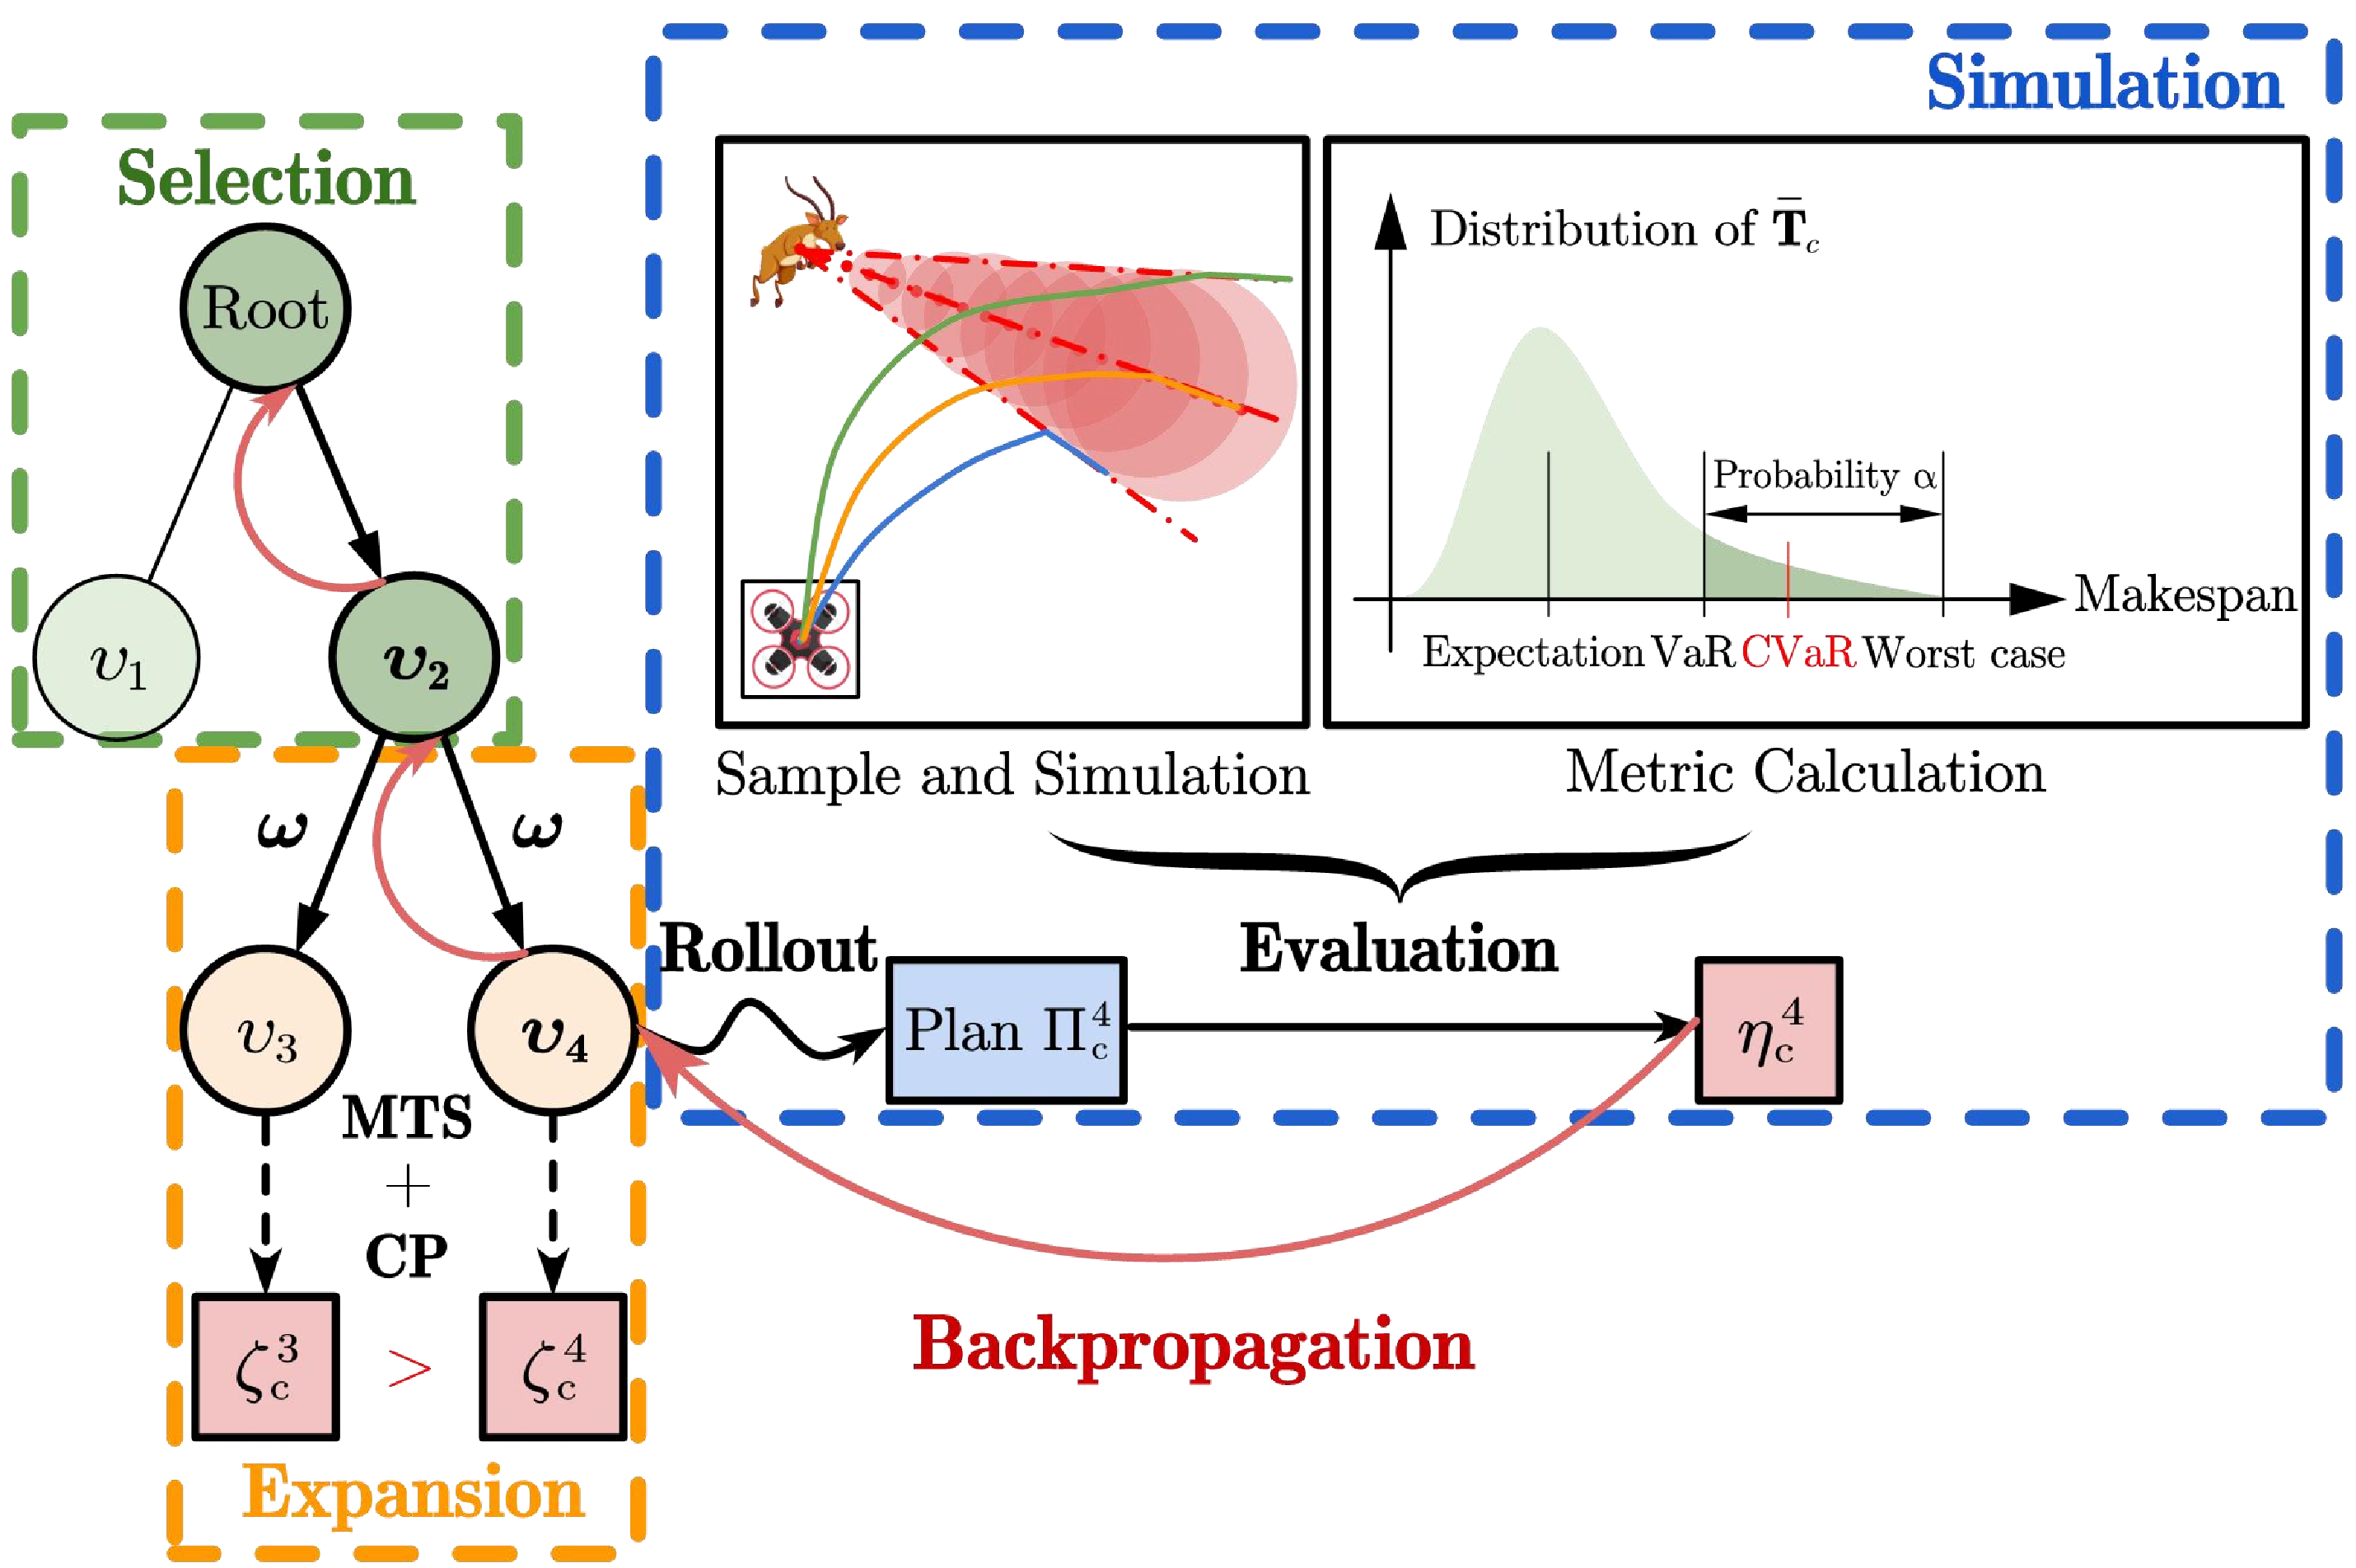
\includegraphics[width=0.95\linewidth]{figures/ch06/CP-MCTS.pdf}
%  \vspace{-2mm}
%  \caption{Procedures of the proposed CP-MCTS in Sec.~\ref{ch06:subsec: assignment}.}
%  \label{ch06:fig:MCTS}
%  \vspace{-0.2in}
%\end{figure}
%%==============================

%=======================================
\subsubsection{CP-based Monte Carlo Tree Search}\label{ch06:sec:cp-mcts}

Monte Carlo Tree Search (MCTS) is a well-known heuristic search algorithm
for solving complex planning problems in dynamic scenes.
Built upon this algorithm, this work introduces CP-based Monte Carlo Tree Search (CP-MCTS).
As summarized in Alg.~\ref{ch06:alg:cp-mcts} and Fig.~\ref{ch06:fig:fra},
it is a centralized task planning algorithm
designed to efficiently
handle complex temporal tasks associated with dynamic targets.
% In particular,
% it iterates through four steps
% over the search space of potential assignments
% until the planning time elapses:
It repeats four stages until the time budget expires:
selection, expansion, simulation, and backpropagation.
Notably, as the number of robots and tasks increases,
the nodes generated during the ``Expansion'' phase grow rapidly.
If ``{Simulation}'' is performed for all expanded nodes,
the algorithm becomes biased toward breadth-first search, neglecting depth exploration and thus reducing efficiency.
To mitigate this, a CP-based metric is introduced to
efficiently evaluate and select the most promising child nodes,
which are then advanced to the ``Simulation'' stage.


\subsubsection{Selection and Expansion}
% A node~$\nu \triangleq (\tau_1,\,\tau_2,\cdots,\tau_N)$
% encodes a partial assignment,
% where $\tau_n$ is the subtask sequence of robot~$n\in \mathcal{N}$.
Each node in the search tree represents a partial assignment of subtasks, i.e.,
$\nu \triangleq (\tau_1,\,\tau_2,\cdots,\tau_N)$,
where $\tau_n$ is the ordered sequence of subtasks assigned
to robot~$n\in \mathcal{N}$.

%=======================================
\setlength{\textfloatsep}{5pt}
\begin{algorithm}[!t]
    \caption{CP-based MCTS \texttt{(CP-MCTS)}}
    \label{ch06:alg:cp-mcts}
    \SetKwInOut{Input}{Input}
    \SetKwInOut{Output}{Output}
    \Input{Robots~$\mathcal{N}$, poset~$P_{\varphi}$, duration func.~$\rho$, \\
	time budget~$t_b$, target estimations~$\widehat{Y}_{\mathcal{H}_t}, {G}_{\mathcal{H}_t}$.}
    \Output{Plan~$\Pi_\texttt{c}^\star$, average makespan~$\eta_\texttt{c}^\star$.}
    Initialize root node $\nu_0$, \(\eta_\texttt{c}^\star \leftarrow \infty\);\\
    \While{$time < t_b$}{
    	% $//$~$Selection$\\
    	Leaf node~$\nu \leftarrow$ \texttt{Selection}($\nu_0$);\\
	Child nodes $\{ \nu_{+}\}$ $\leftarrow$ \texttt{Expansion}($\nu,\, P_{\varphi}$);\\
    Filtered nodes $\{ \nu_\texttt{s}\}$ via $\zeta$ in (\ref{ch06:eq:metric});\\
	\For{$\nu_\texttt{s} \in \{\nu_\texttt{s}\}$}
	{\tcc{Simulation\,=\,Rollout\,+\,Eval}
    $\Pi_\texttt{c} \leftarrow$ \texttt{Rollout}($\nu_\texttt{s},\, P_{\varphi},\, \rho,\, \widehat{Y}_{\mathcal{H}_t},\, x_t$);\\
	$\eta_\texttt{c} \leftarrow \texttt{Eval}(\Pi_\texttt{c},\, P_{\varphi},\, \rho,\, \hat{Y}_{\mathcal{H}_t},\, G_{\mathcal{H}_t},\, x_t)$;\\
	\If{$\eta_\texttt{c} < \eta_\texttt{c}^\star$}
	{$\eta_\texttt{c}^\star \leftarrow \eta_\texttt{c},\, \Pi_\texttt{c}^\star \leftarrow \Pi_\texttt{c}$;\\}
	\texttt{Backpropagate}($\nu_\texttt{s}, \, \xi_\texttt{c}$);\\
	}
    }
\end{algorithm}
%=======================================

During~``{Selection}'',
the Upper Confidence Bound applied to Trees (UCT) \cite{2006Bandit} is used to choose
nodes for ``{Expansion}''.
The UCT value is computed as
$(\overline{\xi}_i+Q\times\sqrt{\frac{ln B}{b_i}})$,
where \(\overline{\xi}_i\) is the estimated value of the \(i\)-th child node,
\(b_i\) is its visit count,
\(B\) is the visit count of the current node,
and \(Q>0\) is a parameter that balances exploration and exploitation.
% Starting from the root, we recursively select the child with the highest UCT until reaching a leaf node.
Starting from the root, at each level the child with the highest UCT value
is recursively selected until a leaf node is reached.


During~``{Expansion}'', unless a terminal state with a complete assignment is reached,
child nodes are generated from the leaf node by assigning the \textit{next} subtask
to the robot team.
Let $\Omega_{\nu}\triangleq \{\omega\in\tau_n,\,\forall n\in \mathcal{N}\}$ be
the set of subtasks already assigned in node~$\nu$,
and $\Omega^-_{\nu} \triangleq \Omega_{\varphi} \backslash \Omega_{\nu}$
the remaining ones.
To ensure feasibility,
the \textit{next} subtask~$\omega$ is chosen from
% $\Omega^-_{\nu}$ while
% ensuring that \textit{all} its preceding subtasks have been assigned, i.e.,
% \begin{equation}\label{ch06:eq:next-task}
$\Omega^{\texttt{a}}_{\nu} \triangleq \big{\{}\omega\, |\, \omega \in \Omega^-_{\nu}, \omega' \in \Omega_\nu, \forall \omega' \in \text{Pre}(\omega)\big{\}}$,
% \end{equation}
where
% $\Omega^{\texttt{a}}_{\nu}$ denotes the set of subtasks that can be assigned for node~$\nu$, and
$\text{Pre}(\omega)$ represents the set of subtasks that must be completed
before~$\omega$ according to R-poset~$P_{\varphi}$.
In other words, a subtask~$\omega_i$ cannot be assigned to node~$\nu$
if some $\omega_j$ with $(\omega_j, \omega_i) \in \preceq_{\varphi}$
has not yet been assigned.
When a subtask~$\omega \in \Omega^{+}_{\nu}$ is selected,
a child node $\nu^+$ is created by assigning $\omega$ to a robot group~$\mathcal{I}_{\omega}$,
i.e., by appending it to the local plan~$\tau_n$ of each robot~$n \in \mathcal{I}_{\omega}$.
For child node~$\nu^+$, define \emph{key subtasks} $\Omega^{\texttt{s}}_{\nu^+}\subset \Omega_{\nu^+}$ as:
% \begin{equation}
% \label{ch06:eq: first-task}
$\Omega^{\texttt{s}}_{\nu^+}\triangleq \big{\{} \omega\,|\,\omega=\tau_{n}[0],
\, \omega \notin \tau_{n'}[1:],\, \forall n,n' \in \mathcal{N}\big{\}}$,
%  \Omega^{1}_{\nu^+}\triangleq \big{\{}\omega|\omega=\tau_{n}[0], \forall n \in \mathcal{N}\big{\}},\\
  % \Omega^{2}_{\nu^+}\triangleq (\tau_{1}/\tau_{1}[0]) \cup \cdots \cup (\tau_{N}/\tau_{N}[0]),
% \end{equation}
where~$\Omega^{\texttt{s}}_{\nu^+}$ contains the first-to-execute subtasks across robots,
independent of others.
Stepwise simulation is then performed based on
the predicted target trajectories~\(\widehat{Y}_{\mathcal{H}_t}\),
as described in the sequel,
resulting in the predicted completion time~$\widehat{T}_{\omega}$
for each assigned subtask~$\omega \in \Omega_{\nu^+}$.

==============================
\begin{figure}[t]
 \centering
 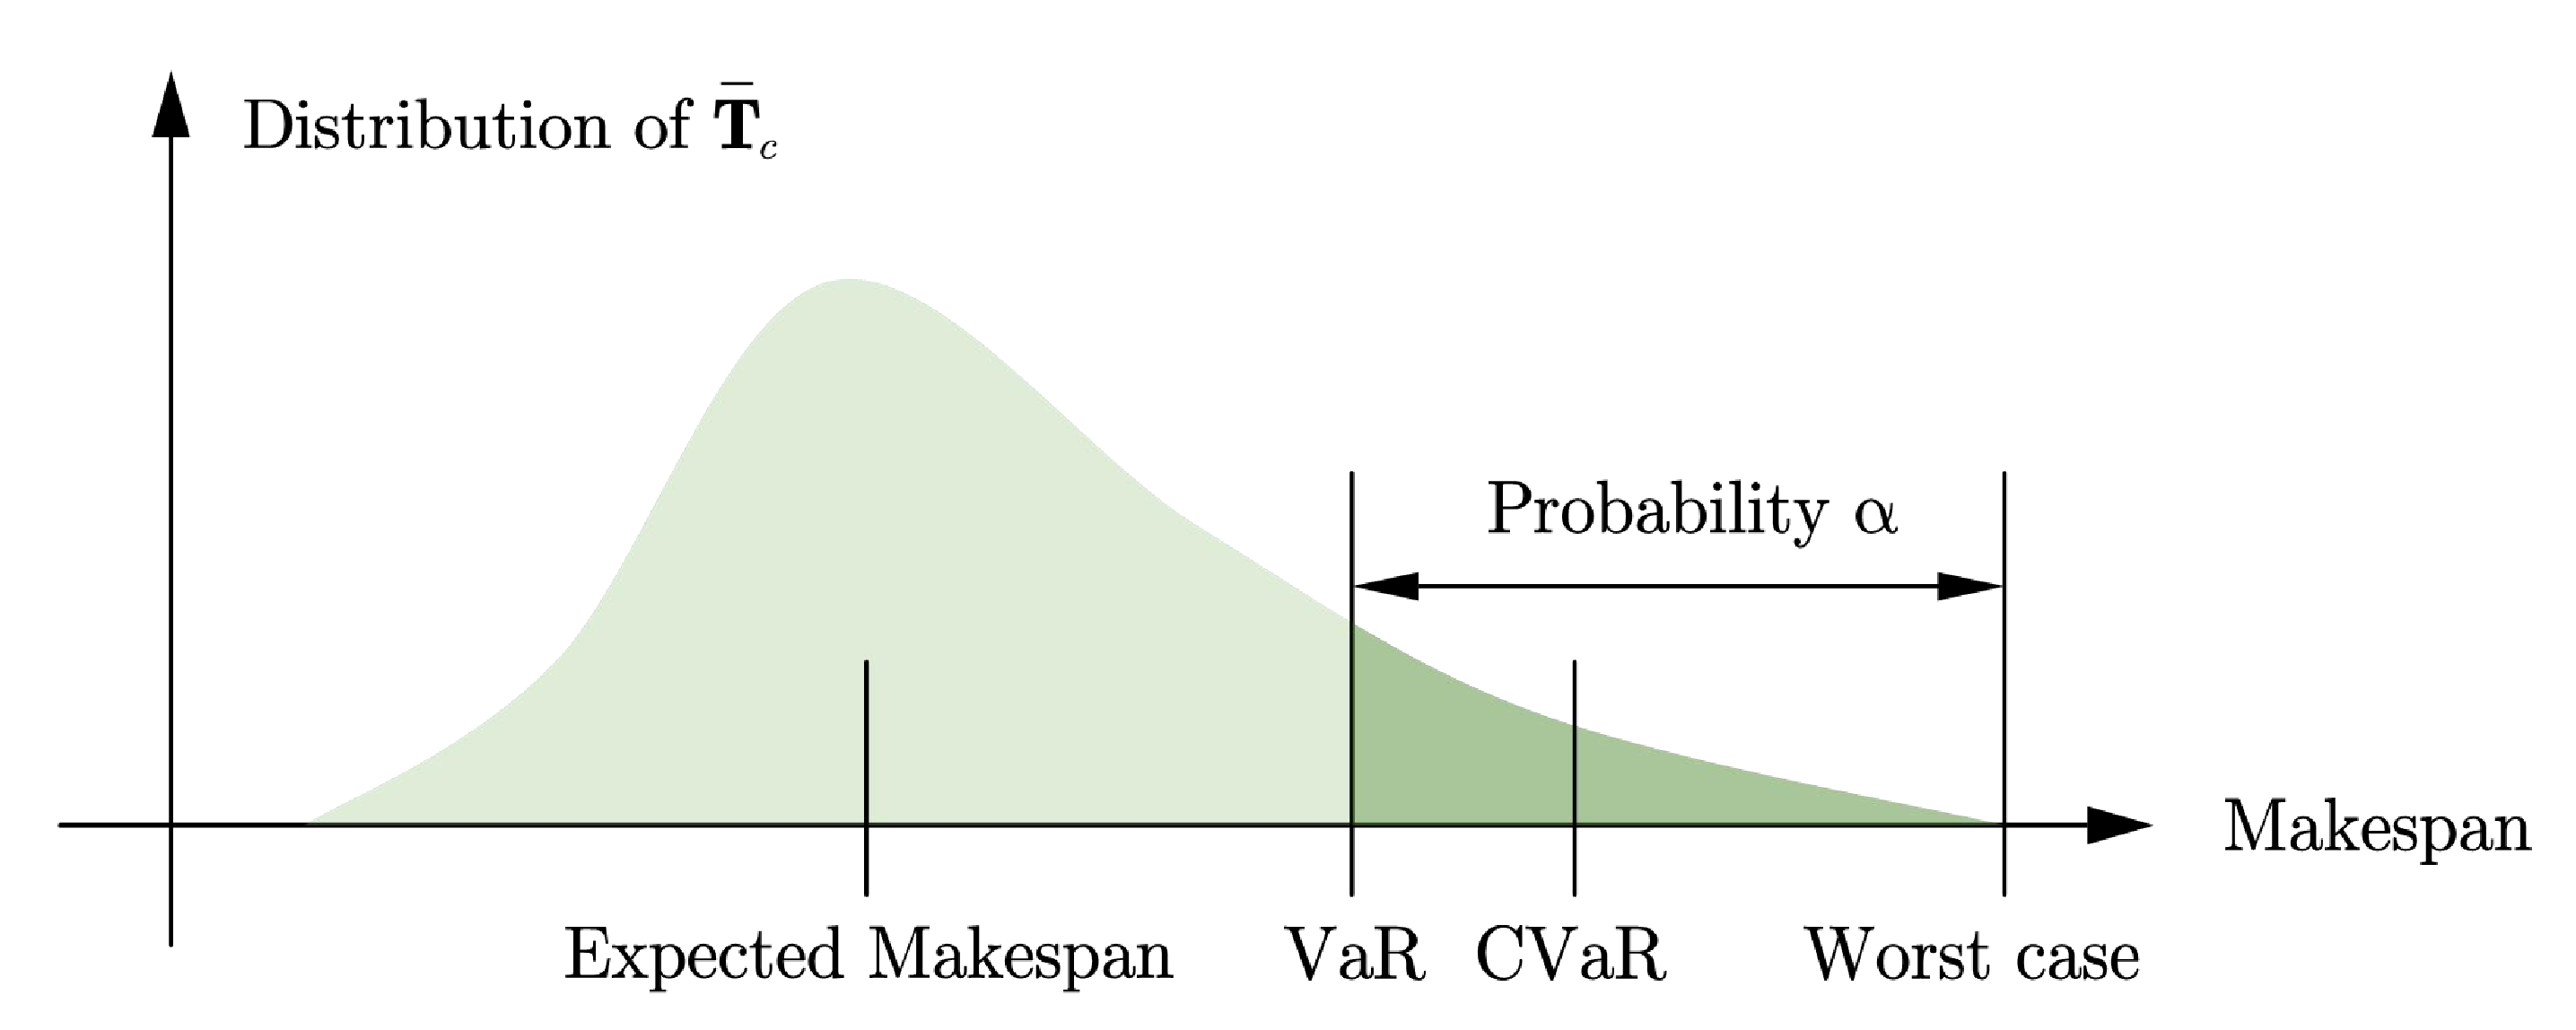
\includegraphics[width=0.95\linewidth]{figures/ch06/CVaR.pdf}
 \vspace{-2mm}
 \caption{Illustration of risk measure: VaR and CVaR.}
 \label{ch06:fig:CVaR}
 \vspace{-1mm}
\end{figure}
==============================


\subsubsection{Simulation}
The ``{Simulation}'' procedure consists of three steps:
(I) \textit{rollout} to complete an assignment;
(II) sample the makespan distribution;
(III) evaluate the plan based on this distribution.
First, a \textit{rollout} policy is applied recursively from the selected child node
until all subtasks are assigned.
In each iteration, the \textit{next} subtask is selected as in ``Expansion''
and assigned to a robot group either randomly
or greedily according to stepwise simulation results.
To enhance \textit{rollout} diversity,
we use a random factor \(\epsilon \in [0, 1]\):
with probability \(\epsilon\),
a feasible robot group is chosen uniformly at random;
with probability \(1-\epsilon\),
the group expected to initiate this subtask earliest is selected.
% This strategy is formally defined as:
% \begin{equation*}
%     \mathcal{I}^{\star} \sim
% \begin{cases}
%     \texttt{Rand} (\boldsymbol{\mathcal{I}_{\omega}}), & \text{with prob}~\epsilon; \\
%     \textbf{argmin}_{\mathcal{I} \in \boldsymbol{\mathcal{I}_{\omega}}}
%     \,T_\omega^\texttt{s}(\nu, \omega, \mathcal{I}, \widehat{Y}_{\mathcal{H}_t}), &  \text{with prob}~(1-\epsilon),
% \end{cases}
% \end{equation*}
% where \(\nu\) is the current node; \(\omega\) represents the subtask to be assigned;
% $\boldsymbol{\mathcal{I}_{\omega}}$ denotes the set of all feasible robot groups;
% \(\mathcal{I}^{\star}\) is the selected group;
% and \(T_\omega^\texttt{s}\) is the estimated subtask starting time,
% computed via stepwise simulation using the predicted target trajectories~\(\widehat{Y}_{\mathcal{H}_t}\).
Once a complete plan~\(\Pi_\texttt{c}\) is obtained,
a sampling-based method derives its average makespan distribution~\(\mathbf{\overline{T}}_\texttt{c}\)
via stepwise simulation with \(z\in \mathbb{N}\) samples drawn
from the prediction regions \(\widehat{Y}_{\mathcal{H}_t}, G_{\mathcal{H}_t}\).
% Specifically, \(z\in \mathbb{N}\) samples \(\{\widetilde{Y}(z)\}\) are drawn from the prediction regions \(\widehat{Y}_{\mathcal{H}_t}, G_{\mathcal{H}_t}\),
% and stepwise simulation is run for each realization to obtain the average makespan distribution
% \(\mathbf{\overline{T}}_\texttt{c}\).
%%==============================
%\begin{remark}\label{ch06:rm:sim}
%It is important to note that as the total makespan increases,
%the stepwise simulation time typically extends,
%resulting in a longer overall task assignment time.
%However, by increasing the simulation time step \(\Delta t\), we can reduce the computational time.
%Experimental results have shown that a moderate increase
%in the step size has minimal impact on the accuracy of the
%estimation results.
%
%\end{remark}
%% ==============================
\begin{definition}[VaR and CVaR]
The value at risk (VaR) at risk level \(\alpha \in (0,1]\)
is defined as $\text{VaR}_{\alpha}(\Pi_\texttt{c}) \triangleq
      {\textbf{inf}}\big\{\rho\in\mathbb{R},\, \text{Prob}(
      \mathbf{\overline{T}}_\texttt{c}\geq\rho)\geq\alpha\big\}$,
i.e., the \(\alpha\)-quantile of the distribution \(\mathbf{\overline{T}}_\texttt{c}\).
The associated conditional value at risk (CVaR) is defined as:
$\text{CVaR}_\alpha(\Pi_\texttt{c})
\triangleq \mathbb{E}\big{[}\mathbf{\overline{T}}_\texttt{c}|
  \mathbf{\overline{T}}_\texttt{c}\geq\mathrm{VaR}_\alpha(\Pi_c)\big{]}$,
as the expected value of the worst \(\alpha\)-quantile of \(\mathbf{\overline{T}}_\texttt{c}\).

\end{definition}


As shown in Fig.~\ref{ch06:fig:fra},
VaR captures the maximum loss at a given confidence level,
while CVaR assesses the expected loss beyond the VaR threshold,
providing a more informative measure of tail risk.
Accordingly, we use \(\eta_\texttt{c}\triangleq \text{CVaR}_{\alpha}(\Pi_\texttt{c})\)
as the evaluation metric for each plan based on its average makespan distribution.
The procedure of deriving the distribution and computing the CVaR
is encapsulated as~\(\texttt{Eval}(\cdot)\).
During the search, the best plan~$\Pi_\texttt{c}^\star$
and its minimal risk value~$\eta_\texttt{c}^\star$ are maintained.
For each new candidate~$\Pi_\texttt{c}$,
if \(\eta_\texttt{c} < \eta_\texttt{c}^\star\),
both $\Pi_\texttt{c}^\star$ and $\eta_\texttt{c}^\star$ are updated.

\subsubsection{Backpropagation}
To support the tree search, we define a normalized performance measure:
\begin{equation}
\xi_\texttt{c} \triangleq 2 - \frac{\eta_\texttt{c}}{\eta_\texttt{c}^\star},
\end{equation}
which facilitates comparison across different branches of the search tree.
During ``{Backpropagation}'',
the evaluation values and visit counts of nodes are propagated and
updated along the path from the selected node to the root.
% \todo{$\xi_\texttt{c}=2 - ({\eta_\texttt{c}}/{\eta_\texttt{c}^\star}$,
% add description and equations.}

% Lastly, the following three task allocation algorithms are adopted to
% evaluate the complete solution during the ``{Simulation}'' process:
% (I) \(\textbf{CVaR}_{\alpha}\): The proposed method, which
%     uses CVaR as the evaluation metric, with \(\alpha\) representing the chosen risk level.
% (II) \textbf{No Trajectory Prediction (NTP)}: Evaluates the plan assuming stationary targets.
% (III) \textbf{No Uncertainty (NU)}: Evaluates the plan by considering only the
% predicted mean trajectory \(\widehat{Y}_{\mathcal{H}_t}\), without accounting for trajectory uncertainty.
%==============================
\begin{lemma}
\textnormal{
Given an expanded node~$\nu^+$,
the completion times of \textit{key subtasks} in $\Omega^{\texttt{s}}_{\nu^+}$
%in~\eqref{ch06:eq: first-task}
satisfy that
$$\text{Pr}\Big(T_{\omega} \leq \widehat{T}_{\omega} + \frac{G_{\widehat{T}_{\omega}, m}}
       {\underset{n \in \mathcal{I}_{\omega}}{\textbf{min}}\{v_n\}-v^{\star}_{m}}, \Big.
\Big. \forall \omega \in \Omega^{\texttt{s}}_{\nu^+} \Big) \geq (1-\delta)^{|\Omega^{\texttt{s}}_{\nu^+}|},$$
where $T_{\omega}$ is the actual completion time of subtask~$\omega\in \Omega^{\texttt{s}}_{\nu^+}$;
$m$ is the associated target;
$\mathcal{I}_{\omega}$ is the set of robots executing~$\omega$;
$v_{n}$ and $v^{\star}_{m}$ are the velocities of robot $n$ and target $m$.}
\end{lemma}
\begin{proof}
% \todo{check whether variables are defined after revision.}
From the simulation results,
all robots $n \in \mathcal{I}_{\omega}$ assigned to subtask $\omega \in \Omega^{\texttt{s}}_{\nu^+}$
would reach the predicted position
$\widehat{Y}_{\widehat{T}_{\omega}, m}$ of target~$m$
by time instance~$\widehat{T}_{\omega}$.
By the probability guarantee in~\eqref{ch06:eq:cpg}, it holds that
$$\text{Pr}\Big(\left\| Y_{\widehat{T}_{\omega}, m} - \widehat{Y}_{\widehat{T}_{\omega}, m} \right\|
\leq G_{\widehat{T}_{\omega}, m}, \Big.
\Big. \forall \omega \in \Omega^{\texttt{s}}_{\nu^+} \Big)
\geq (1 - \delta)^{|\Omega^{\texttt{s}}_{\nu^+}|}.$$
%where~$\Omega^{\texttt{s}}_{\nu^+}$ is the set of subsequent subtasks to be executed
%in~\eqref{ch06:eq: first-task} in node~$\nu^+$.
The additional delay required to reach target~$m$ is upper-bounded by
%\begin{equation*}
$\widehat{T}_\omega^{\texttt{e}} = {G_{\widehat{T}_\omega, m}}
/({{\textbf{min}_{n \in \mathcal{I}_{\omega}}}\{v_n\} -v^{\star}_{m}})$,
%\end{equation*}}
this completes the proof.
%
\end{proof}

==============================
\begin{figure}[t!]
  \centering
  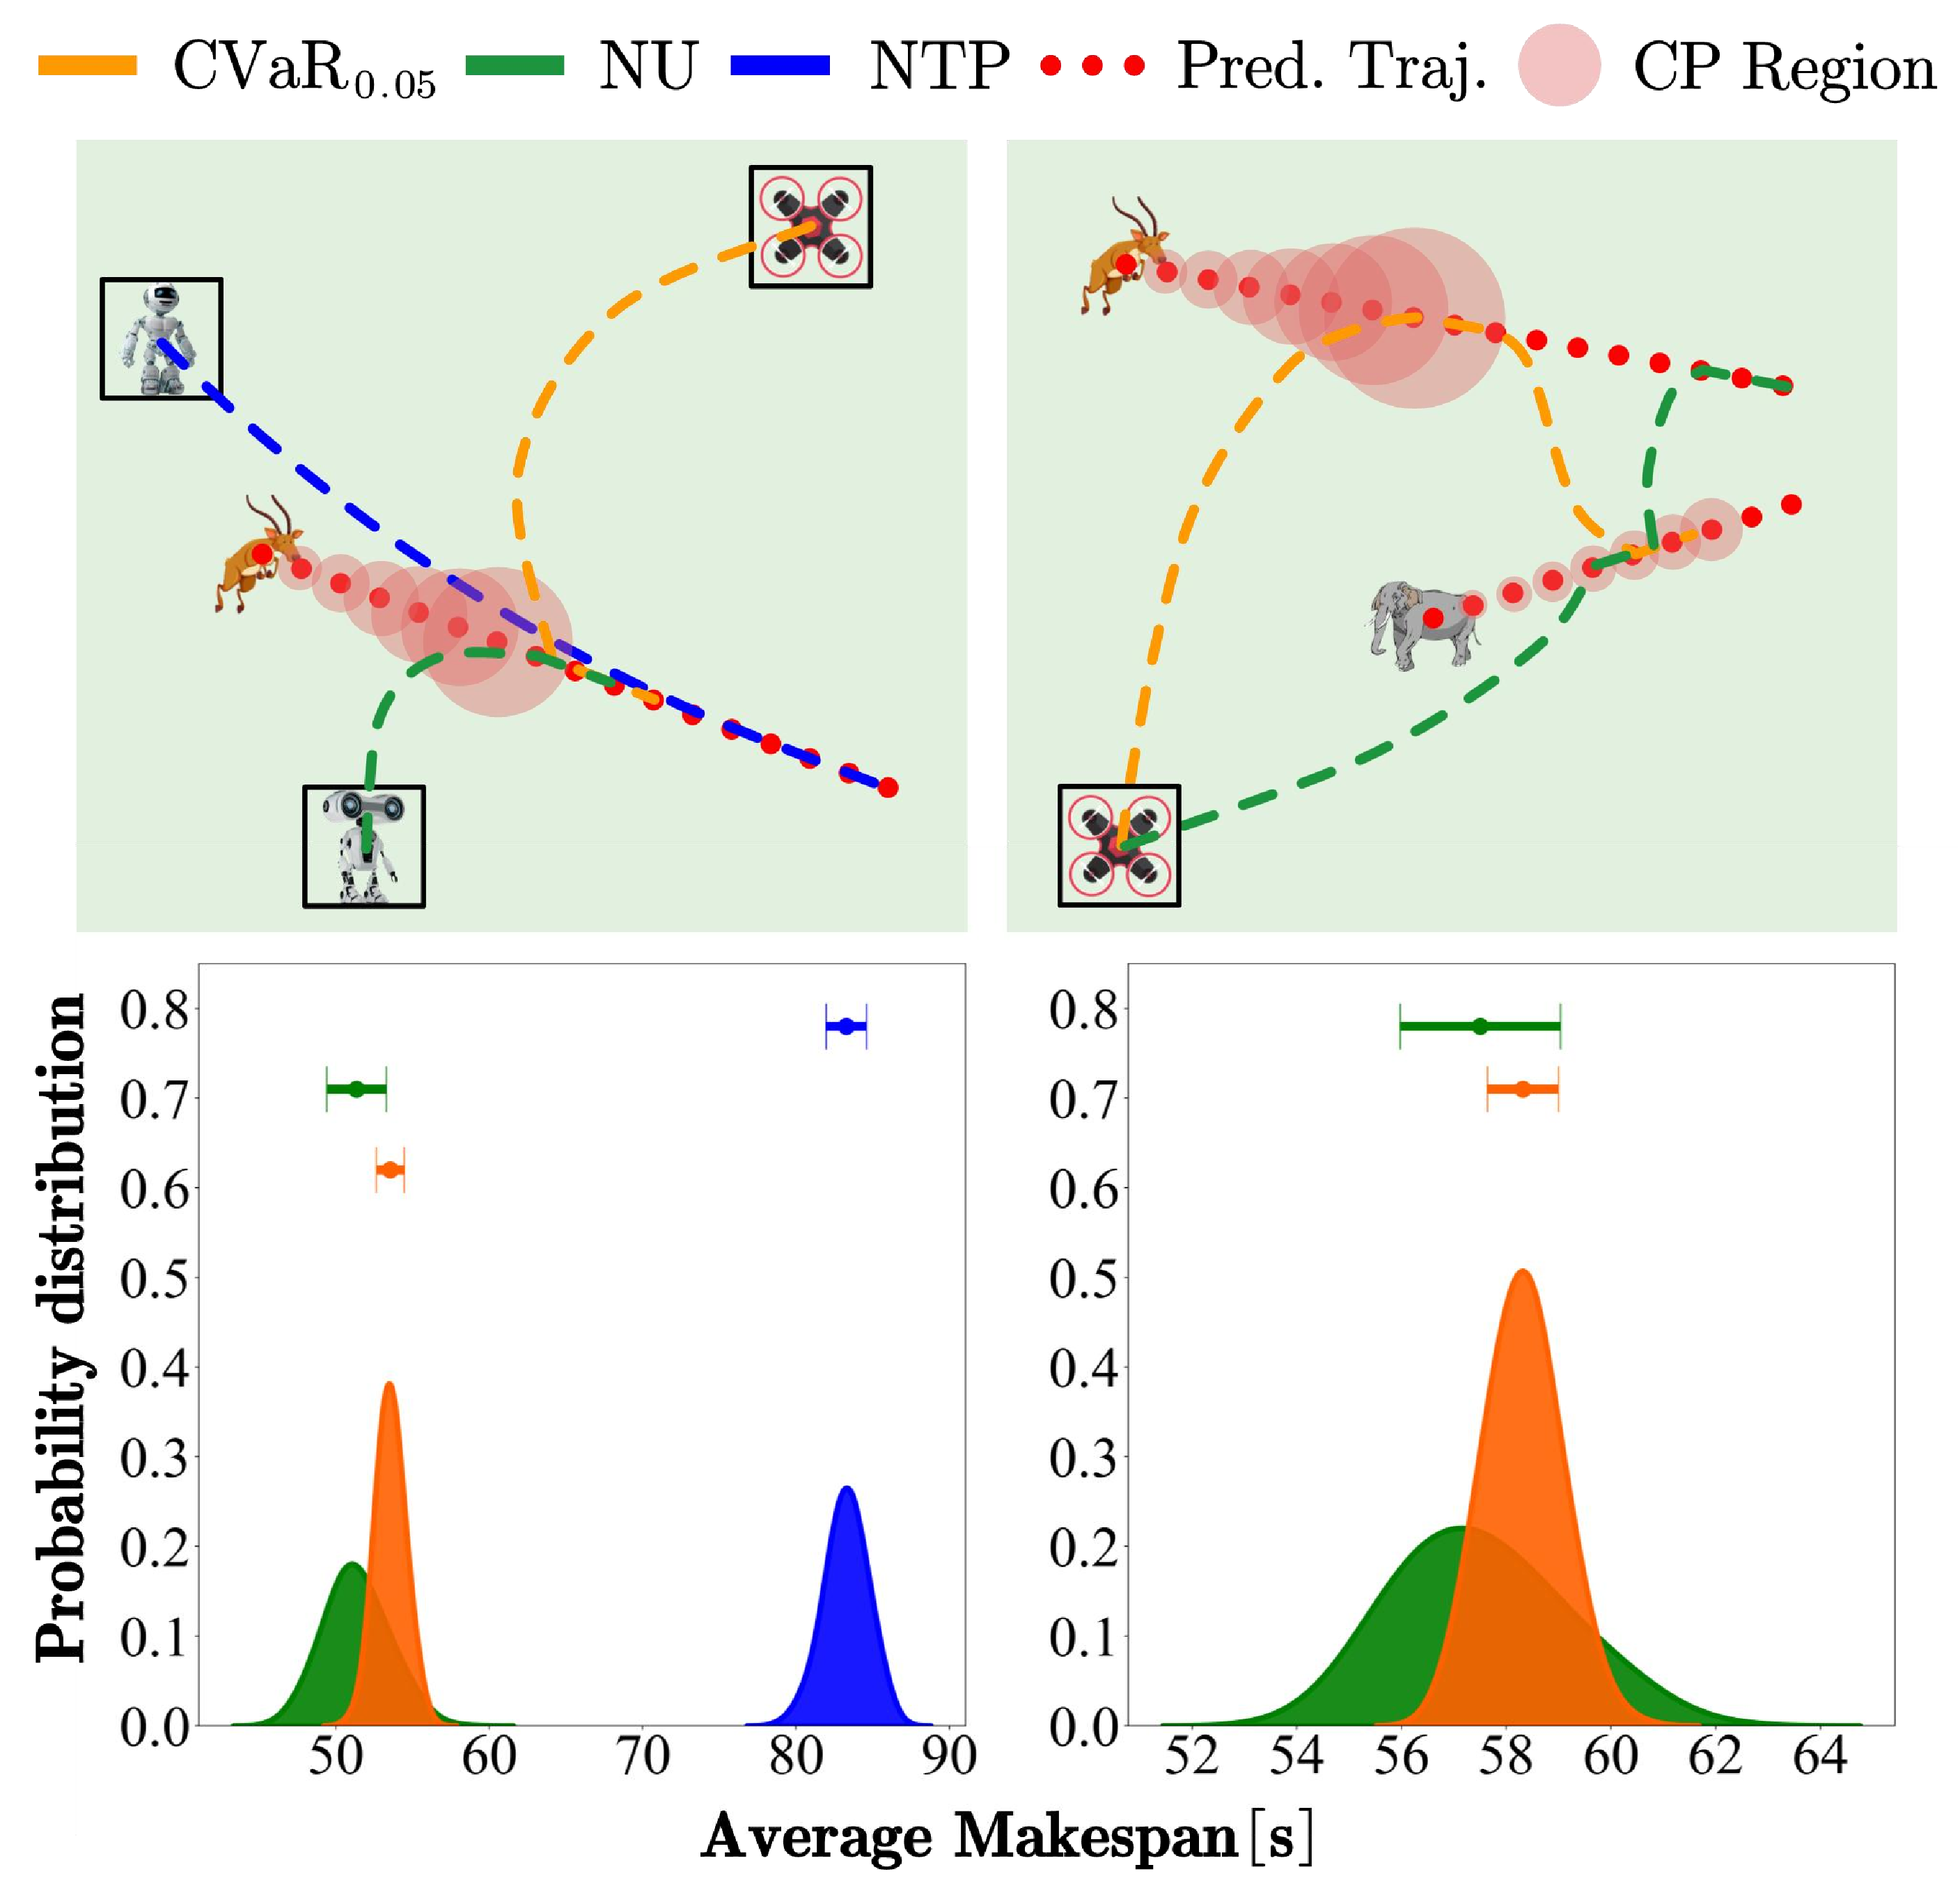
\includegraphics[width=2.6in]{figures/ch06/offline_cases.pdf}
  \vspace{-2mm}
  \caption{Comparison of different methods in two scenes.
  \textbf{Top:} Final trajectories;
  \textbf{Bottom:} Distribution of the makespan given the assignments.}
  \label{ch06:fig:offline_cases}
  \vspace{-1mm}
\end{figure}
==============================

The actual completion time of a first executed subtask~\(T_{\omega}\)
is probabilistically bounded by the predicted time \(\widehat{T}_{\omega}\)
plus an uncertainty term determined by the prediction region~\(G_{\widehat{T}_{\omega}, m}\)
and the velocity difference between the slowest robot and the target.
Hence, with confidence level \((1-\delta)\),
each \textit{key subtask} completion time can be reliably estimated.
The evaluation metric for a child node~$\nu^+$ is then defined as:
\begin{equation}
\label{ch06:eq:metric}
\zeta_{\nu^+} \triangleq \frac{\sum_{i=1}^{|\Omega_{\nu^+}|}\widehat{T}_{\omega_i}  + \sum_{j=1}^{|\Omega^{\texttt{s}}_{\nu^+}|} \widehat{T}_{\omega_j}^\texttt{e} }{|\Omega_{\nu^+}|},
\end{equation}
which approximates the average completion time of assigned subtasks with uncertainty adjustment.
After ``Expansion'', for each \textit{next} subtask, the child node with the smallest~$\zeta$ is selected to enter ``{Simulation}'',
forming the filtered set~$\{\nu_\texttt{s}\}$.

%==============================
\begin{remark}\label{ch06:rm:velocity}
For a child node $\nu^+$, if a subtask $\omega \in \Omega^{\texttt{s}}_{\nu^+}$
is assigned to a
robot~$n \in \mathcal{I}_{\omega}$ with velocity~$v_n \leq  v^{\star}_{m}$,
the robot may be unable to complete the subtask.
In this case, the predicted completion time is $\widehat{T}_{\omega} = \infty$,
which yields $\zeta_{\nu^+} = \infty$;
thus the node is excluded from the ``Simulation'' step.
\end{remark}
% ==============================


==============================
\begin{remark}\label{ch06:rm:eval-sim}
  Besides the proposed \(\text{CVaR}_{\alpha}\) approach,
  two alternative task allocation algorithms are used in the ``{Simulation}'' phase
  to evaluate complete plans:
  (I) {No Trajectory Prediction (NTP)},
  which assumes stationary targets;
  (II) {No Uncertainty (NU)}, which considers
  predicted trajectories \(\widehat{Y}_{\mathcal{H}_t}\)
  but ignores uncertainty regions \(G_{\mathcal{H}_t}\).
  {Comparative results for two simple scenes are presented in Fig.~\ref{ch06:fig:offline_cases}.
  It can be seen that \(\text{CVaR}_{0.05}\) achieves a lower mean makespan than NTP by accounting for target motion,
  and exhibits greater risk aversion than NU,
  as evidenced by its reduced variance due to the incorporation of trajectory uncertainty.}
  % In particular, in the left scene, \(\text{CVaR}_{0.05}\)
  % selects the fastest UAV to monitor the antelope,
  % leveraging its higher speed to mitigate uncertainty in task completion time.
  % In the right scene,
  % the algorithm prioritizes the antelope-related task,
  % as the antelope's high velocity leads to rapid growth in trajectory uncertainty;
  % thus, \(\text{CVaR}_{0.05}\) aims to complete the task as early as possible to reduce risk.

\end{remark}
==============================

% \begin{example}
% \label{ch06:offline_cases}
% Fig. \ref{ch06:fig:offline_cases} illustrates the results of two simple scenes.
% In scene-3, the task is to choose between two GRs or a UAV to monitor an antelope.
% The NTP method assigns GR1 (green trajectory), initially closest to the antelope, but its mininal speed
% difference results in a longer catch-up time.
% The NU method assigns GR2 (blue trajectory),
% while the \(\textbf{CVaR}_{0.05}\) method opts for the UAV (orange trajectory),
% despite a higher expected makespan,
% as its higher speed reduces uncertainty in task completion time.

% In scene 4, a UAV must decide the order of monitoring an antelope and an elephant.
% Due to speed differences, uncertainty in the antelope's predicted
% trajectory grows faster than for the elephant.
% The NU method prioritizes the elephant, whereas the \(\textbf{CVaR}_{0.05}\) method reverses this order, prioritizing the antelope to minimize uncertainty in the average makespan.
%
% \end{example}

%==============================
\subsection{Online Execution and Adaptation}\label{ch06:subsec: execution}
\subsubsection{Online Execution and Adaptation}
%=======================================
\setlength{\textfloatsep}{5pt}
\begin{algorithm}[!t]
    \caption{Online Dynamic Task Assignment}
    \label{ch06:alg:ta}
    \SetKwInOut{Input}{Input}
    \SetKwInOut{Output}{Output}
    \Input{Robots \(\mathcal{N}\),\, task formula~$\varphi(t)$,\, duration func.~$\rho$,\,
    	      trajectory predictors $\mathbf{\Upsilon}$,\, prediction regions $G_{\mathcal{H}_t}$,\,
              observations $\{Y_{0:t}, V_{0:t}\}$.}
    \Output{Assignment~$\Pi^\star$.}
    Initialize \(P_{\varphi}\) \(\leftarrow \texttt{Compute\_poset}(\varphi(0))\),\,
    \( \Omega_\iota \leftarrow \emptyset\); \\
    Initialize \(\Pi^\star, \, \eta^\star \leftarrow \texttt{CP-MCTS}(P_{\varphi}, \rho,
    \hat{Y}_{\mathcal{H}_0}, G_{\mathcal{H}_0}, x_0)\);\\
    % Set \(\Omega_\iota = \emptyset\);\\
    \While{not terminated}
        {
        Each robot \(n \in \mathcal{N}\) applies \(\pi_n\);\\
        Sense $x_{t}$ and $Y_{t}$;\\
        Obtain predictions $\hat{Y}_{\mathcal{H}_t}$;\\
%        Update \(\{\widehat{\mathbf{y}}_m(t)\}\) by (\ref{ch06:eq:estimation});\\
        Update \(\varphi(t)\) by (\ref{ch06:eq:task-update});\\
        Update \(P_{\varphi}\) by \(\texttt{Compute\_poset}(\varphi(t))\);\\
        \If{\(\varphi_{\texttt{r}}(t)\)}
        {
             \(\Pi^\star,\, \eta^\star\) \(\leftarrow\) \texttt{CP-MCTS}(\(P_{\varphi}, \rho, \hat{Y}_{\mathcal{H}_t}, G_{\mathcal{H}_t}, x_t\));\\
        }
        \Else{
       	 \(\eta^\star \leftarrow \eta^\star - 1\);\\
            \If{\(\Omega_{\texttt{c}}(t) \neq \emptyset\)}
            {
                Update \(\eta^\star\) by (\ref{ch06:eq:update_eta});\\
                \(\Omega_\iota \leftarrow \Omega_\iota \cup \Omega_\texttt{c}(t)\);\\
            }
            \(\eta^\star_t\leftarrow \texttt{Eval}(\Pi^\star, P_{\varphi}, \rho, \hat{Y}_{\mathcal{H}_t}, G_{\mathcal{H}_t}, x_t)\);\\
            \If{\(\eta^\star_t > (1+\gamma)\eta^\star\)}
            {
                \(\widehat{\Pi}_t, \, \widehat{\eta}_t \leftarrow \texttt{CP-MCTS}(P_{\varphi}, \rho, \hat{Y}_{\mathcal{H}_t}, G_{\mathcal{H}_t}, x_t)\);\\
                \If{\(\widehat{\eta}_t < \eta^\star_t\)}
                {
                    \(\Pi^\star \leftarrow \widehat{\Pi}_t,\, \eta^\star \leftarrow \widehat{\eta}_t\);\\
                }
            }
            }
        \(t \leftarrow t+1;\)
    }
\end{algorithm}
%=======================================

As illustrated in Fig.~\ref{ch06:fig:fra} and summarized in Alg.~\ref{ch06:alg:ta},
the planning scheme consists of two stages:
initial planning and online adaptation.
Following the initial plan,
each robot \(n \in \mathcal{N}\) executes its local plan~\(\pi_n\)
by navigating to the targets specified by the assigned subtasks
and then performing the corresponding actions.
When executing action~\(a^{K_n}_n\) on target~\(m^{K_n}_n\),
the robot~$n$ must wait for collaborators
if \(a^{K_n}_n\) belongs to a multi-robot collaboration~$C_k$ (i.e., \(|C_k|>1\)).
Such partial synchronization is essential to handle uncertainties in navigation and task execution times.
If the action is non-collaborative,
the robot proceeds independently without waiting.
% Robots synchronize only for collaborations; otherwise they execute actions independently.

At each time step \(t>0\),
the robot states $x_t$ and target observations~$Y_t$ are updated,
and new predictions~$\hat{Y}_{\mathcal{H}_t}$ are generated from $Y_{0:t}$
using the trajectory predictors~$\mathbf{\Upsilon}$.
Moreover, the task formula \(\varphi(t)\) is updated
by integrating triggered reactive task formula, i.e.,
\begin{equation}
\label{ch06:eq:task-update}
    \varphi(t) \triangleq \varphi(t^-)
  \wedge \varphi_{\texttt{r}}(t),
\end{equation}
where \(\varphi(t^-)\) is the previous formula
and \(\varphi_{\texttt{r}}(t)\triangleq \bigwedge_{\bar{e}\in \bar{E}}
 \Diamond\varphi_\texttt{rep}^{\bar{e}}(t)\) is the reactive tasks released at time~$t$.
The current R-poset \(P_{\varphi}\) is updated accordingly.
Replanning is triggered under two conditions:
(I) new reactive tasks appear, i.e., $\varphi_{\texttt{r}}(t) \neq \emptyset$, or
(II) the current plan's performance degrades significantly, i.e.,
$\eta^\star_t > (1+\gamma)\eta^\star$, where $\gamma \in (0,1)$ is the replanning triggering ratio.
Here, the performance metric $\eta^\star_t$ is computed via \(\texttt{Eval}(\cdot)\)
given the latest observations.
For completed tasks,
the expected value $\eta^\star$ is updated as
\begin{equation}
\label{ch06:eq:update_eta}
\eta^\star_{+} \triangleq \frac{\big{(}|\varphi(t)| - |\Omega_\iota|
  +|\Omega_{\texttt{c}}(t)|\big{)}}  {|\varphi(t)| - |\Omega_\iota|} \eta^\star_{-},
\end{equation}
where $\eta^\star_{+}$ and $\eta^\star_{-}$ denote the updated and previous values;
$|\varphi(t)|$ is the total number of tasks;
$|\Omega_\iota|$ is the number of completed tasks;
and $|\Omega_{\texttt{c}}(t)|$ is the number of tasks finished at time $t$.
When replanning is triggered, CP-MCTS generates a candidate plan $\widehat{\Pi}_t$ with metric $\widehat{\eta}_t$.
The system adopts this new plan only if it offers improved performance as $\widehat{\eta}_t < \eta^\star_t$.
Otherwise, the current plan $\Pi^\star$ is maintained and
the metric $\eta^\star$ is monotonically decreased to reflect progress.
This procedure repeats until the system terminates.



%=======================================
\subsubsection{Complexity Analysis}
The computational complexity of Alg. \ref{ch06:alg:ta} is analyzed as follows.
Generating a R-poset has worst-case complexity \(\mathcal{O}(J^2)\), where \(J\) is the number of subtasks,
bounded by the number of edges in the NBA.
% The size of the NBA is double exponential in $|\varphi|$.
For task assignment, the worst-case search space
is \(\mathcal{O}(J!\cdot N^J)\),
as subtask orderings are combinatorial and
assignments grow exponentially with the number of robots~$N$.
In contrast, the \textit{rollout} process remains
\(\mathcal{O}(J\cdot N)\), as subtasks are assigned randomly or greedily.
The complexity of stepwise simulation is \(\mathcal{O}(\frac{z T\cdot(J+N)}{\Delta t})\),
where \(z\) is the number of samples, \(T\) is the makespan
and \(\Delta t\) is the time step.


%=======================================
\subsubsection{Generalization}
There are two notable extensions of the proposed scheme.
\textit{(I) Robot Failures}.
In the event of robot failures,
a modified {CP-MCTS} is employed to generate a new plan.
The root node is updated to exclude failed robots and include completed subtasks.
If a failure occurs during execution,
the affected subtask is rescheduled.
The standard CP-MCTS procedure is then applied to update the assignment.
% the ``Expansion'' step selects the remaining tasks under
% the same ordering constraints, followed by
% ``Simulation'' and ``Backpropagation'' to update the assignment.
\textit{(II) Dynamic Task Priority}.
When tasks are associated with different priorities~\(\alpha_\ell\),
the optimization objective shifts from the average makespan~$\overline{T}_{\varphi}$
to the weighted makespan~$\widetilde{T}_{\varphi} \triangleq \sum_{\ell=1}^{L_t} \alpha_\ell T_{\varphi_\ell}$,
which emphasizes high-priority tasks.
% \improve{\todo{(III) Addition and Removal of Targets}}
